\chapter{Použitý model}\label{model}

Jelikož úloha uvedená v kapitole \ref{problem} je úlohou, v níž je adresa URL rozdělena na části, a ty jsou posléze rozděleny na tokeny, je na model použitý k aproximaci klasifikační funkce kladen požadavek, aby reflektoval tuto hierarchickou strukturu vstupních dat. Použitý model využívá přístupu pomocí multi-instančního učení \footnote{resp. jeho speciální varianty, popsané v kapitole \ref{MIL-modification}.}, popsaného v kapitole \ref{MIL}, aplikovaného dvakrát na sebe sama. Tím je umožněno modelovat nejprve tři vybrané části adresy URL (doménu, cestu a dotaz) z jejich tokenů, a následovně z těchto tří částí modelovat samotnou adresu URL. V následující kapitole je předpokládána základní znalost fungování umělých neuronových sítí v rozsahu prvních dvou částí \cite{goodfellow_deep_2016}.

\section{Reprezentace adresy URL pomocí tašek vektorů}\label{URL_MIL_representation}
V kapitole \ref{problem} byla definována abeceda \( \Sigma \) všech znaků přípustných v adrese URL. Každý token adresy URL je slovem nad touto abecedou. Neuronové sítě, které byly použity, však potřebují vstup v podobě vektoru čísel, dále zvaného \BPname{vektor příznaků} (\BPenname{feature vector}). K tomu je použita funkce \( \psi \), projektující tokeny do prvků eukleidovského prostoru \( \BPfield R^n \). Tím je definován prostor všech vektorů příznaků jako
\[ \BPspace X_1 = \psi \left( \Sigma^* \right) \subset \BPfield R^n \]
kde \( \Sigma^* \) značí množinu všech slov nad abecedou \( \Sigma \). Prostor \( \BPspace B_1 \subset \BPspace P^M \left( \BPspace X_1 \right) \) je konstruován tak, že každá taška v \( \BPspace B_1 \) odpovídá vektorům příznaků tokenů jedné části jedné adresy URL. Za použití paradigmatu vloženého prostoru, popsaného v kapitole \ref{embedded-space-paradigm}, lze najít nějakou vkládající funkci
\[ \phi_1 : \BPspace B_1 \to \BPspace X_2 \]
kde \( \BPspace X_2 \) je opět nějaký vstupní prostor, který může, ale nemusí být totožný s \( \BPspace X_1 \). Nad tímto prostorem je konstruován prostor tašek \( \BPspace B_2 \subset \BPspace P^M \left( \BPspace X_2 \right) \) tak, že každá taška v prostoru \( \BPspace B_2 \) odpovídá vektorům příznaků tří částí jedné adresy URL. Opětovným použítím paradigmatu vloženého prostoru lze nalézt vkládající funkci
\[ \phi_2 : \BPspace B_2 \to \BPspace X_3 \]
kde \( \BPspace X_3 \) je opět nějaký vstupní prostor, který obecně nemusí být totožný s prostory \( \BPspace X_1 \) a \( \BPspace X_2 \). Tím je celá adresa URL vyjádřena jedním vektorem příznaků z prostoru \( \BPspace X_3 \). Celá tato konstrukce je graficky znázorněna na obrázku \ref{url_model_MIL}.

\begin{figure}[h]
	\centering
	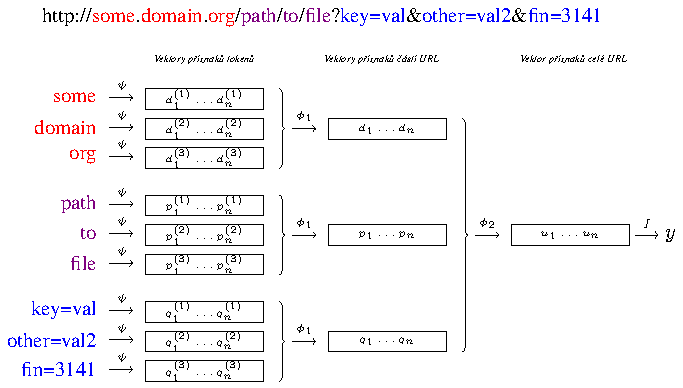
\includegraphics{images/model_MIL/model_MIL.pdf}
	\caption{Model adresy URL}\label{url_model_MIL}
\end{figure}

\section{Modifikace MIL pro tuto úlohu}\label{MIL-modification}
Každá adresa URL musí obsahovat doménu, ale i adresy, kterým chybí cesta nebo dotaz (nebo dokonce cesta i dotaz), mohou být validními adresami URL ve smyslu \cite{berners-lee_uniform_1994}. Vzhledem k tomu, jak byl prostor \( \BPspace B_2 \) konstruován, je tedy zřejmé, že platí
\[ \left( \forall b \in \BPspace B_2 \right) \left( 1 \leq \left| b \right| \leq 3 \right) \]
Chybějící části adresy URL je ale možné reprezentovat jedním tokenem odpovídajícím prázdnému slovu\footnote{Což nutně nemusí znamenat, že jsou reprezentovány nulovým vektorem příznaků.} abecedy \( \Sigma \). Díky tomuto rozšíření lze předchozí odhad velikosti tašek v prostoru \( \BPspace B_2 \) zesílit na
\[ \left( \forall b \in \BPspace B_2 \right) \left( \left| b \right| = 3 \right) \]

Protože doména, cesta a dotaz mají v adrese URL fundamentálně odlišný účel, nedává smysl, aby jim odpovídající vkládající funkce byly totožné. Rozšíření multi-instančního přístupu navržené v předchozím odstavci umožňuje nahradit funkci \( \phi_1 \) třemi různými vkládajícími funkcemi \( \phi_D \), \( \phi_P \) a \( \phi_Q \), odpovídajícími doméně, cestě a dotazu respektive. Rovněž předpis pro vkládající funkci \( \phi_2 \) se díky konstantní velikosti tašek z prostoru \( \BPspace B_2 \) zjednoduší na
\[ \phi_2 : \BPspace X_2^3 \to \BPspace X_3 \]
Takto modifikovaná abstrakce je graficky znázorněna na obrázku \ref{url_model_modified_MIL}.

\begin{figure}[h]
	\centering
	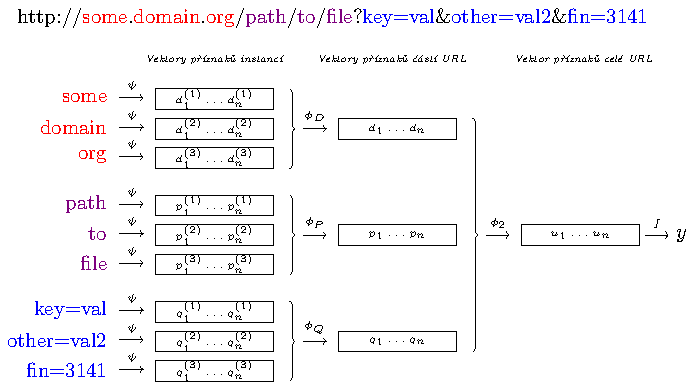
\includegraphics{images/model_modified_MIL/model_modified_MIL.pdf}
	\caption{Modifikovaný model adresy URL}\label{url_model_modified_MIL}
\end{figure}

\section{Metody hledání vkládající a klasifikační funkce}
Obecně lze v multi-instančním učení definovat vkládající funkci \( \phi \) jako
\begin{equation}\label{netpooling}
	\phi : \BPspace B \to \bar{\BPspace X} : b \mapsto g \left( \left\{ k \left( x \right) \middle| x \in b \right\} \right)
\end{equation}
kde
\begin{align*}
	k &: \BPspace X \to \BPfield R^l \\
	g &: \bigcup_{m = 1}^{+ \infty} \left( \BPfield R^l \right)^m \to \bar{\BPspace X}
\end{align*}
Za \( g \) lze volit například funkce minimum, maximum, aritmetický průměr. Funkce \( k \) je realizována neuronovou sítí, která je trénována libovolným algoritmem pro učení s učitelem. Pokud jsou funkce \( k \) a \( f \) obě realizovány neuronovou sítí, jsou tyto neuronové sítě trénovány společně.

V dalším textu budou předpokládány již konkrétní prostory, a sice
\begin{align*}
	\BPspace X_1 &= \BPfield R^n \\
	\BPspace X_2 &= \BPfield R^n \\
	\BPspace X_3 &= \BPfield R^{3n} \\
	\BPspace Y &= \left\{ -1, +1 \right\}
\end{align*}
pro nějaké \( n \in \BPfield N \).

Přístup pomocí \eqref{netpooling} byl využit pro vkládající funkce první úrovně, tedy
\begin{align*}
	\phi_D &: \BPspace B_1 \to \BPfield R^n : b \mapsto g_D \left( \left\{ k_D \left( x \right) \middle| x \in b \right\} \right) \\
	\phi_P &: \BPspace B_1 \to \BPfield R^n : b \mapsto g_P \left( \left\{ k_P \left( x \right) \middle| x \in b \right\} \right) \\
	\phi_Q &: \BPspace B_1 \to \BPfield R^n : b \mapsto g_Q \left( \left\{ k_Q \left( x \right) \middle| x \in b \right\} \right)
\end{align*}
Za vkládající funkci druhé úrovně byla volena funkce konkatenace vektorů, tedy funkce \( \phi_2 : \left( \BPfield R^n \right)^3  \to \BPfield R^{3n} \) s funkčním předpisem
\begin{multline}
	\phi_2 \left( \left( x_1^{(1)}, \dots, x_n^{(1)} \right), \left( x_1^{(2)}, \dots, x_n^{(2)} \right), \left( x_1^{(3)}, \dots, x_n^{(3)} \right) \right) = \\
	= \left( x_1^{(1)}, \dots, x_n^{(1)}, x_1^{(2)}, \dots, x_n^{(2)}, x_1^{(3)}, \dots, x_n^{(3)} \right)
\end{multline}
Takto lze vkládající funkci \( \phi_2 \) volit pouze díky modifikaci navržené v kapitole \ref{MIL-modification}.

Klasifikační funkce \( f : \BPfield R^{3n} \to \left\{ -1, +1 \right\} \) je realizována neuronovou sítí, která je trénována společně s neuronovými sítěmi realizujícími funkce \( k_D \), \( k_P \) a \( k_Q \).

Takto navržené vkládající funkce neberou v potaz pořadí objektů v jednotlivých taškách. Díky své relativní jednoduchosti byl zvolen tento přístup, přestože pořadí objektů v taškách má vliv na výsledný klasifikátor (srov. \cite{vinyals_order_2015}).

\section{Použité přenosové funkce}
V modelech požitých k řešení úlohy popsané v kapitole \ref{problem} byly použity čtyři typy neuronů s různými \BPname{přenosovými funkcemi} (\BPenname{activation function}).

\subsection{Lineární přenosová funkce}
Jedním z nejjednoduších typů neuronů je neuron s lineární přenosovou funkcí, mající pro vstup neuronu \( x \) tvar (bez váhy a vychýlení)
\[ f : \BPfield R \to \BPfield R : x \mapsto x \]

\subsection{ReLU}
Neurony typu \BPname{ReLU} (\BPenname{Rectified linear unit}) používají přenosovou funkci (bez váhy a vychýlení), která pro vstup neuronu \( x \) dává výstup
\[ f : \BPfield R \to \BPfield R : x \mapsto \max \left\{ 0, x \right\} \]

\subsection{Maxout}
Pro neurony typu \BPname{maxout} (srov. \cite{goodfellow_maxout_2013}) nelze přenosovou funkci definovat stejně jednoduše jako v případě neuronů typu ReLU. Přenosová funkce \( h \) v tomto případě nebývá definována pro jednotlivé neurony, ale pro celou vrstvu neuronů po složkách \( h_i : \BPfield R^n \to \BPfield R \) jako funkce (včetně váhy \( \BPmat W \) a vychýlení \( b \))
\[ h_i \left( x \right) = \max_{j \in \left[ 1, k \right]} z_{ij} \]
kde
\[ z_{ij} = x^T \BPmat W_{\cdot ij} + b_{ij} \]
kde
\[ \BPmat W \in \BPfield R^{n, m, k} \qquad b \in \BPfield R^{m, k} \]
Lze tedy vrstvu maxout chápat jako \( k \) lineárních vrstev, z nichž je vybráno maximum výstupů.

\subsection{Softmax}
Přenosová funkce pro neurony typu \BPname{softmax} je také definována pro celou vrstvu po složkách \( h_i : \BPfield R^n \to \BPfield R \) jako funkce (bez váhy a vychýlení)
\[ h_i \left( x \right) = \frac{e^{x_i}}{\sum_{j = 1}^n e^{x_j}} \]
Výhodou této přenosové funkce pro její využití spolu s objektivní funkcí popsanou v kapitole \ref{loss_function} je její jednoduchá derivace tvaru
\[ \frac{\partial h_i}{\partial x_j} = \begin{cases}
	h_i \left( 1 - h_i \right) \quad \text{pro} \quad i = j \\
	-h_i h_j \quad \text{jinak}
\end{cases} \]

\section{Použitá objektivní funkce}\label{loss_function}
Při využití neuronů s přenosovou funkcí softmax jako poslední vrstvy neuronové sítě lze za objektivní funkci položit funkci, která pro parametry modelu \( \theta \), vstupní vektor \( x \) a skutečnou třídu \( y \) maximalizuje věrohodnostní funkci
\[ \mathcal L \left( \theta \middle| y, x \right) \]
Tuto věrohodnostní funkci lze zapsat jako sdruženou pravděpodobnost, kterou naopak lze zapsat pomocí podmíněné pravděpodobnosti, tedy platí
\[ \mathcal L \left( \theta \middle| y, x \right) = P \left( y, x \middle| \theta \right) = P \left( y \middle| x, \theta \right) P \left( x \middle| \theta \right) \]
Pro pevné hodnoty parametrů \( \theta \) tedy platí
\[ \mathcal L \left( \theta \middle| y, x \right) = P \left( y \middle| x \right) = \prod_{i = 1}^n P \left( y_i \middle| x \right)^{y_i} \]
Hodnota \( P \left( y_i \middle| x \right) \) je v poslední vrstvě aproximována neurony typu softmax s přenosovou funkcí \( h_i \), tedy je maximalizována hodnota
\[ \prod_{i = 1}^n h_i^{y_i} \]
Úloha maximalizace této hodnoty je ekvivalentní úloze minimalizace jejího záporného logaritmu. Je tedy minimalizována hodnota takto definované funkce \( J \), dané předpisem
\[ J = -\log \prod_{i = 1}^n h_i^{y_i} = -\sum_{i = 1}^n y_i \log h_i \]
Funkce \( J \) je nazývána \BPname{objektivní funkcí minimalizující cross-entropii}. V případě binární klasifikace (\( n = 2 \)) lze tuto funkci zapsat jako 
\[ J = - y_i \log h_i - \left( 1 - y_i \right) \log \left( 1 - h_i \right) \]

Výhodou objektivní funkce minimalizující cross-entropii je její jednoduchá derivace tvaru
\[ \frac{\partial J}{\partial x_i} = h_i - y_i \]

Celá tato podkapitola byla zpracována podle \cite{roelants_how_2017}.

\section{Metody trénování neuronových sítí}
Jednou ze základních metod trénování neuronových sítí je metoda \BPname{gradientního sestupu} (srov. \cite{cauchy_methode_1847}). Předpokládá se existence nějaké objektivní funkce \( J \left( \theta \right) \), jejíž minimum je hledáno. \( \theta \in \BPfield R^d \) jsou učené parametry modelu. Tyto parametry se opakovaně mění, dokud není nalezeno požadované minimum funkce \( J \). V metodě gradientního sestupu jsou nové parametry \( \hat \theta \) počítány pomocí vztahu
\[ \hat \theta = \theta - \eta \nabla_{\theta} J \left( \theta \right) \]
kde \( \eta \) je krok učení.

Při použití metody \BPname{stochastického gradientního sestupu} je tato korekce prováděna pro každou dvojici vstupního objektu \( x \) a výstupního objektu \( y \), tedy jde o metodu tvaru
\[ \hat \theta = \theta - \eta \nabla_{\theta} J \left( \theta; x, y \right) \]
Výhodou této metody je efektivita učení při velkém množství trénovacích dat, na druhou stranu je její nevýhodou velká fluktuace hodnot objektivní funkce.

Kompromisem mezi základním gradientním sestupem a stochastickým gradientním sestupem je metoda \BPname{mini-batch gradientního sestupu}. Tato metoda je srovnatelně efektivní jako stochastický gradientní sestup při vyšší stabilitě hodnot objektivní funkce. Při použití metody mini-batch gradientního sestupu je z dostupných vstupních a výstupních objektů vybírána podmnožina zvaná \BPname{mini-batch} a jsou určovány nové parametry jako
\[ \hat \theta = \theta - \eta \nabla_{\theta} J \left( \theta; x^{\left( i, \dots, i + n \right)}, y^{\left( i, \dots, i + n \right)} \right) \]

Metoda gradientního sestupu je základem pro mnoho moderních metod trénování neuronových sítí (srov. \cite{duchi_adaptive_2011}, \cite{zeiler_adadelta:_2012}, \cite{tieleman_lecture_2012} a \cite{kingma_adam:_2014}). Použitá metoda je další metodou založenou na gradientním sestupu.

\BPname{ADAM} (srov. \cite{kingma_adam:_2014}) je variantou stochastického gradientního sestupu s proměnlivým krokem učení. K správnému nastavení tohoto kroku je v této metodě přenášena hodnota gradientu a jeho čtverce mezi jednotlivými kroky. Metoda ADAM je parametrizována třemi parametry \( \beta_1 \), \( \beta_2 \) a \( \varepsilon \). V každém kroku \( t \) jsou počítány momenty
\[ m_t = \beta_1 m_{t - 1} + \left( 1 - \beta_1 \right) \nabla_{\theta} J \left( \theta \right) \]
\[ v_t = \beta_2 v_{t - 1} + \left( 1 - \beta_2 \right) \left( \nabla_{\theta} J \left( \theta \right) \right)^2 \]
Vzhledem k tomu, že počáteční hodnoty jsou \( m_0 = 0 \) a \( v_0 = 0 \), bylo by učení zpočátku velice pomalé. Tomu lze předejít použitím opravných hodnot
\[ \hat{m_t} = \frac{m_t}{1 - \beta_1^t} \]
\[ \hat{v_t} = \frac{v_t}{1 - \beta_2^t} \]
Nové hodnoty parametrů modelu jsou nalezeny jako
\[ \hat \theta = \theta - \frac{\eta \hat{m_t}}{\sqrt{\hat{v_t}} + \varepsilon} \]
\cite{kingma_adam:_2014} navrhují hodnoty parametrů metody
\[ \beta_1 = 0.9 \qquad \beta_2 = 0.999 \qquad \varepsilon = 10^{-8} \]

Metoda ADAM byla vybrána z důvodů použití adaptivního kroku učení, vedoucího ke stabilnější výsledné hodnotě a počáteční rychlosti díky využití opravných hodnot. Mezi další výhody patří jednoduché použití díky dobře fungujícím hodnotám parametrů, které byly navrženy autory metody.
